\chapter{Approach}
\label{chap:approach}
In this chapter we discuss some design decisions of our solution such as 
platform choice, as well as a formal overview of our implementation. 

In the following the term client is used to refer to a web browser.


\section{Choice of Platform}
\label{sec:platform}
There are many different techniques to implement a web-based application. 
The problem specifies that the solution must be able  on the one hand to 
communicate with LDBN 
and on the other hand to extend some of its capabilities, 
thus a basic HTML solution will not be able to achieve our goal, 
since all pages in that case are static. 

The remaining options can be divided into 3 groups, client-side, server-side and
a client-server based. 

The client-side solutions consist of a Java applet or a Flash
application which are downloaded to the browser and then run on the user's computer
using a browser plugin. However, this approach has the disadvantage
of requiring a plug-in, which is not always available by default on all web browsers...

Server-side includes solutions built in PHP, ASP, ASP.NET, C/C++ or
Perl, all which is ran on the server and then sent to the user's browser as
a static HTML page. With this approach the client is unable to remember its state and 
every user interaction caused an HTTP round trip over the network, 
requiring browsers to re-render the whole web page after each request...

The third one is
a client-server based idea called Asynchronous JavaScript and XML (AJAX),
which is also used by the initial version of LDBN. 
It works almost the same as the server-side solutions but acts more interactively. The
reason for this is that some parts of the program logic are moved form the server
to the client, thus not every user interaction causes neccasaryly a whole new page
to be rendered. Instead with AJAX the client can request 
data from the server in the background, i.e. without the need to freeze the user interface. 
This is usually done by XMLHttpRequest API, which is implemented
by the browser. The API can be accessed by the application using JavaScript, it can be
used to handle communication with the server in an asynchronous fashion over a
simple HTTP connection.
This way after the data is received the client can change only the affected parts of the web page. 
This on the other hand is once again done by JavaScript, which 
can be used to access and manipulate the Document Object Model (DOM) of the web page.
An example of an AJAX architecture is illustrated in Figure~\ref{fig:ajax01}, 
which is an adaption of~\cite[Figure 3.1]{mt1}.

\begin{figure}[h]
	\begin{center}
		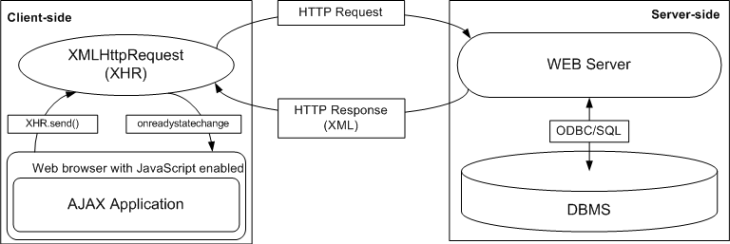
\includegraphics[width=0.8\textwidth]{./img/ajax01a.png}
		\caption{Example of an AJAX Architecture}
		\label{fig:ajax01}
	\end{center}
\end{figure}


It should be noted that AJAX has several shortcomings as well. First of all, 
JavaScript must be enabled in the browser, otherwise the application will not start.
However, the developer can indicate this in the \verb=<noscript>= HTML-tag. 
Nevertheless, the biggest issue with AJAX remains the fact that it is not a
standard. This often requires writing a different code base for different
browsers, and this means less scalability for the application and less productivity for
the developers~\cite{bgwt2}. In the latter case we could avoid some of the issues by using 
Google Web Toolkit (GWT).

\subsection{GWT}
\label{sec:gwt}

GWT is an open source project
and it is developed by Google. It is a set of tools and libraries that allows web developers to
create AJAX applications in Java. 

Some more comments on GWT ....

\subsection{Bitmap Rendering with JavaScript}
\label{sec:renderingJS}
When it comes to visualization and graphics in general we need a 
to have a more low level pixel control over a certain area of the screen. 
When using JavaScript, however, simple tasks such as drawing a straight
line can become quite challenging in a web browser environment.
Of course for this purpose we could use client-side solutions, e.g., using Flash, or 
server-side solution, e.g., rendering everything on the server and sending it back
to the client as a image, but for the same reasons as described in the previous
section we decided to use the AJAX approach. This way we can also
adopt a lot of the source code from the previous version of LDBN. 
One way to achieve bitmap rendering with JavaScript is by
using the \verb=<canvas>= HTML-element. 
It is part of the HTML5~\cite{html5} standard, which is the next major revision of HTML, and it is supported by
most of the modern web browsers. It provides an image-like 
graphics context which can be accessed via a set of JavaScript calls, 
similar to a 2D subset of OpenGL. 
It was originally introduced by Apple in their Safari browser, but it is now 
supported by other modern browser including Mozilla Firefox, Opera and Google Chrome.
It also have  better rendering speed than the older Scalable Vector Graphics (SVG) standard~\cite{w8}. 
Internet Explorer (IE) does not 
provide native support for 
neither SVG nor canvas, though~\cite{w9}. In spite of that, IE does 
implements its own XML-based language for producing vector graphics 
called Vector Markup Language (VML). With the help of VML canvas specific JavaScript 
calls can be emulated in IE. In LDBN we use the GWT-Incubator project~\cite{gwtincubator}, which provides
browser independent canvas implementation for GWT projects, thus 
it provides support for all major browsers including IE. 
It should be noted that by doing this
we loose some rendering speed in IE that generally comes in other browsers
with a native canvas implementation, on the other hand in our implementation of the visualization of FDs we use only static scenes, i.e., 
no animation or any other intensive 
graphical operations, therefore in our opinion VML is sufficient 
for the project. 

\section{Implementation}
\label{sec:implementation}
As mentioned earlier the implementation could be divided into two parts: 
(1) Visualization of FDs and 
(2) improving the existing capabilities of the system.

\subsection{Visualization of FDs}
\label{sec:visualization}
On the one hand the visualization of FDs is the most significant 
part of the thesis, 
on the other hand this extension should not compromise the existing 
user interface of LDBN. Therefore we decided to
make the visualization available in a separate window in the browser. 
The visualization is then available for every field in LDBN which 
contains a set of FDs. These fields contain an eye icon (
\includegraphics[scale=0.6]{./img/eye.png}) in the upper right
corner by clicking it we can open the visualization.
The initial idea
was to implement it as a separate web application, which can then be 
opened in its own 
browser pop-up window. However, there are two problems with this approach. The fist one is
the fact that most of the modern browsers have a pop-up blocker and it is activated by default.
This could have a major negative impact on the usability of the system because there
is always a risk that the user might not notice the pop-up 
warning at all and hence the visualization. The second problem with this approach is 
the fact that we want the visualization to use the existing 
advanced capabilities of LDBN such as drag and drop. This is nearly impossible, thought, since
the two application will run in different JavaScript virtual machines in each
browser window. The a way around this issue could be the use of a server
which communicates with both applications. However, 
this will make the drag and drop too slow for a proper usage. 



In our implementation we use a different approach. We have implemented our own 
JavaScript-based window package.
With it we can create pop-up windows which exists within a browser window. 
An example of such a window is presented in Figure~\ref{fig:fd-visual-win}. 
Our approach eliminates the previously described problems. First,
the window is part of our JavaScript application and as such it does not 
trigger any bowser pop-up
blockers. Second, the visualization and the LDBN system can directly share any 
JavaScript objects, since they run in the same virtual machine, 
this way they can interact in a very fast and efficient way. 
This is very similar to the pop-up dialogs in the initial version of LDBN. 
These dialogs are provided in the standard widget library of GWT. 
However, they prove to be inconvenient for our needs, since once created and attached 
to the DOM they cannot be resized. We on the other hand
need this kind of resize-window functionality since we want to offer to the user
different zoom levels for the visualization, as well as the ability the user to resize the
visualization window, since they could become quite large and hide important parts of the user 
interface. Furthermore, with our implementation we have more powerful control over
the graphical representation of the window, this way for example we can add a close button (image)
in the upper right corner, which is a more intuitive way to interact with the UI.

\begin{figure}[h]
	\begin{center}
		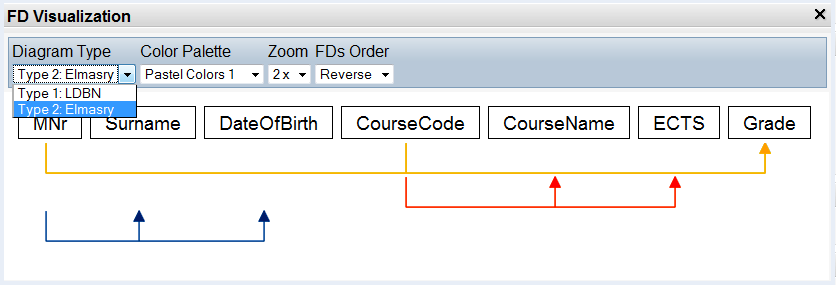
\includegraphics[width=0.8\textwidth]{./img/fd-visual-win.png}
		\caption{FD Visualization Window}
		\label{fig:fd-visual-win}
	\end{center}
\end{figure}

At implementation level the visualization consists of two components. 
Both of them are illustrated in Figure~\ref{fig:impl-fds01}.
The fist component is a simple GWT panel where all the attributes are displayed. Internally 
the attributes are represented as GWT widgets, thus the rendering of those attributes is
handled by the browser. In fact, these are the same widget classes used for representing
attributes in the \emph{Given Attributes} field, which is shown in Figure~\ref{fig:given-atts}. The only 
difference between the two attribute representations is 
that we apply a different CSS style for each of them. By using the already implemented LDBN 
widget classes we get advanced functionality such as drag and drop for free. Thus the users
can drag any attribute in the visualization window and drop 
dropped in the text box of the different editors in LDBN
such as the \emph{Attribute Editor} or the \emph{FD Editor}, the latter is 
shown in Figure~\ref{fig:fdeditor}. 
As a result of which the
attributes are automatically inserted in the text areas of the editor and users do not have
to type them by hand, which for long attribute names could become inconvenient and error-prone. 
We believe the drag and drop functionality can help
users define attributes, keys or FDs much more quickly, which on the other hand can
help improve the usability of the learning environment.

\begin{figure}[h]
	\begin{center}
		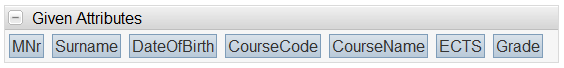
\includegraphics[width=0.8\textwidth]{./img/given-atts.png}
		\caption{Given Attributes Widget}
		\label{fig:given-atts}
	\end{center}
\end{figure}

\begin{figure}[h]
	\begin{center}
		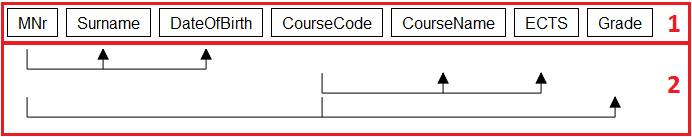
\includegraphics[width=0.8\textwidth]{./img/impl-fds01.png}
		\caption{Visualization Components}
		\label{fig:impl-fds01}
	\end{center}
\end{figure}

\begin{figure}[h]
	\begin{center}
		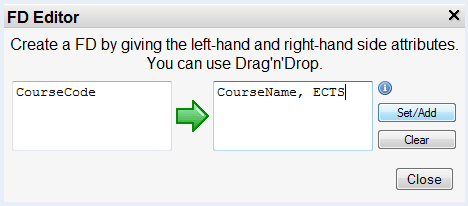
\includegraphics[width=0.6\textwidth]{./img/fdeditor.png}
		\caption{FD Editor Dialog in LDBN}
		\label{fig:fdeditor}
	\end{center}
\end{figure}

The second component of the visualization consists of a \verb=<canvas>= element, it is shown in Figure~\ref{fig:impl-fds01}-2.
The canvas element is placed bellow the attributes, and there the actual drawing 
of the FDs takes place. In LDBN we support two types of visualization, each of them can be selected
from the \emph{Diagram Type} drop dawn menu in the visualization window. The fist type is called 
\emph{Elmasty}, since it is common in~\cite{bdb1}. The main difference between this approach and
the traditional representation of FDs is the fact the we display each attribute in the set of 
FDs only once. 
Similar to the purely text-based representation we can visualize the set
of FDs as a set of rows. Each row representing one FD of the set. 
However, in this visualization all attributes that occur in the set of FDs
are shown in the fist row. Then every FD is displayed in a separate row by a outgoing 
arrow for each attribute from the left-hand side (LHS) of the FD 
and as an incoming arrow for the attributes of the right-hand side (RHS).

This approach is quite intuitive and we believe it will be well received by
students, since during their Database courses at the university most of 
them get familiar with~\cite{bdb1}, from which
the visualization is inspired. However, the approach has some disadvantages
as well. Not the least of which is the fact that it does not make use
of all the available white space in the diagram. To address this issue
we offer a option where the user can change the order in which
the FDs are rendered. In addition to this, we also offer another type of
visualization where the arrows of each FD always start/reach the 
attributes at the top of the diagram. 
Both types of visualization can be observed in 
Figure~\ref{fig:dia_example_elmasry} and~\ref{fig:dia_example_ldbn}.

\begin{figure}[h]
  \centering
  \subfigure[Type: Elmasry]{
    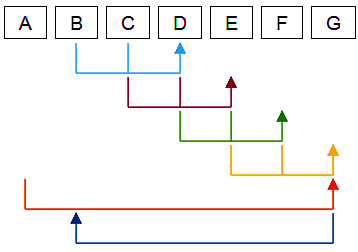
\includegraphics[scale=0.44]{./img/dia-elmasri-ex-fds-01.png}
    \label{fig:dia_example_elmasry}
  }
  \subfigure[Type: LDBN]{
    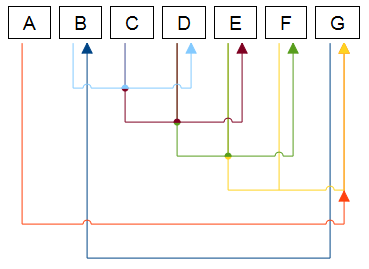
\includegraphics[scale=0.41]{./img/dia-ldbn-ex-fds-01.png}
    \label{fig:dia_example_ldbn}
  }
\caption{Diagram Types in LDBN}
\end{figure}

Another important aspect in visualization in general are certainly colors.
In our visualization we offer five different color palettes. The user can 
choose between:
\begin{enumerate}
	\item \emph{Black Only} - All FDs appear black. This is useful for printing
	purposes.
	\item \emph{Gray Shades} - Each FD appear in several tones of gray. 
	At this point is should be noted that the human eye can detect 
	about 30 shades of gray on a modern LCD screen, 
	which is more than shades of other 
	colors~\cite[Chapter 2]{bimg1} . 
	\item \emph{Pastel Colors} - Here we use less saturated colors which appear pastel. 
	Colors codes are taken from~\cite{wpastel}.
	\item \emph{Standard Colors} - The standard color palette consists of predefined
	HTML colors such as reg, green, blue, etc. These colors often aper vivid 
	(highly saturated colors).
	\item \emph{OpenOffice Style} - With this  palette we use colors which
	can be found in charts created with OpenOffice.org. 
\end{enumerate}
 
% Color Contrast 
% see http://snook.ca/technical/colour_contrast/colour.html
% http://www.w3.org/WAI/WCAG20/quickref/#qr-visual-audio-contrast-contrast
% http://www.w3.org/TR/2008/NOTE-WCAG20-TECHS-20081211/G18

Another important issue when using colors is contrast. 
According to the W3C guidelines a web application should use such
foreground and a background colors that provide enough of a
contrast "when viewed by someone having color deficits or when viewed on a black and white screen"~\cite{w3c1}.
To ensure these property we use WCAG 2.0 contrast ratio formula~\cite{w3c2}.
Our color palettes are WCAG 2 AA Compliant for text larger than 18pt.

As can be seen on Figure~\ref{fig:fd-visual-win}, 
the visualization offers a magnification function as well. 
Thus the user can zoom in and out on a diagram.
This is practical especially when a
diagram contains a lot of attributes and the user 
wants to get a general idea of the FDs, then she/he can
simply zoom out.  
The zoom functionality
is achieved by applying different CSS with different font 
size for the attributes and by redrawing the canvas element accordingly. 

\subsection{Improving LDBN}
\label{sec:improving}

Another major part of this thesis is the improvement of the
existing functionality of the learning environment. 
During the Fall term of 2008,
LDBN was used in conjunction with the course Principles of Database Systems at the
Department of Computing Science at Ume� University, and some important observations
were made. Some of the issues we have 

